\documentclass[11pt]{article}

\usepackage{abstract}
\usepackage{algorithm}
\usepackage{algorithmic}
\usepackage{amsmath}
\usepackage{amssymb}
\usepackage{bm}
\usepackage{caption}
\usepackage{CJKutf8}
\usepackage{color}
\usepackage{enumitem}
\usepackage{epsfig}
\usepackage{fancyhdr}
\usepackage{float}
\usepackage{graphics}
\usepackage{graphicx}
\usepackage{geometry}
\usepackage{indentfirst}
\usepackage{lastpage}
\usepackage{listings}
\usepackage{mathdots}
\usepackage{mathpazo}
\usepackage{multirow}
\usepackage{pstricks-add}
\usepackage{pst-blur}
\usepackage{subcaption}
\usepackage{tikz}
\usepackage{wasysym}
\usepackage{xcolor}
\usepackage[BoldFont,SlantFont,CJKsetspaces,CJKchecksingle]{xeCJK}



\allowdisplaybreaks
\DeclareMathOperator*{\argmin}{argmin}
\definecolor{Blue}{rgb}{1.,0.75,0.8}
\definecolor{mygray}{rgb}{0.5,0.5,0.5}
\definecolor{mygreen}{rgb}{0,0.6,0}
\definecolor{mymauve}{rgb}{0.58,0,0.82}
\pagestyle{empty}
\parindent 2em   %段首缩进
\setlength{\parindent}{2em}
\setCJKmainfont[BoldFont=SimHei]{SimSun}
\setCJKmonofont{SimSun}% 设置缺省中文字体
\usetikzlibrary{arrows, automata, calc, shapes}

\newcommand{\HRule}{\rule{\linewidth}{0.5mm}}
\newcommand{\hytt}[1]{\texttt{\hyphenchar\font=\defaulthyphenchar #1}}
\renewcommand{\algorithmicrequire}{\textbf{Input:}}   
\renewcommand{\algorithmicensure}{\textbf{Output:}}  
% \hyphenation{read-Sym-bol re-ad-Space-Tab-New-line str-Tab}

%\footnotesize
\lstset{ %
  backgroundcolor=\color{white},   % choose the background color; you must add \usepackage{color} or \usepackage{xcolor}
  basicstyle=\ttfamily,            % the size of the fonts that are used for the code
  breakatwhitespace=false,         % sets if automatic breaks should only happen at whitespace
  breaklines=true,                 % sets automatic line breaking
  captionpos=b,                    % sets the caption-position to bottom
  commentstyle=\ttfamily\color{mygreen},    
                                   % comment style
  deletekeywords={},               % if you want to delete keywords from the given language
  escapeinside={},                 % if you want to add LaTeX within your code
  extendedchars=true,              % lets you use non-ASCII characters; for 8-bits encodings only, does not work with UTF-8
  frame=single,                    % adds a frame around the code
  keepspaces=true,                 % keeps spaces in text, useful for keeping indentation of code (possibly needs columns=flexible)
  keywordstyle=\color{blue},       % keyword style
  language=C++,                    % the language of the code
  morekeywords={},                 % if you want to add more keywords to the set
  numbers=left,                    % where to put the line-numbers; possible values are (none, left, right)
  numbersep=5pt,                   % how far the line-numbers are from the code
  numberstyle=\tiny\color{mygray}, % the style that is used for the line-numbers
  rulecolor=\color{black},         % if not set, the frame-color may be changed on line-breaks within not-black text (e.g. comments (green here))
  showspaces=false,                % show spaces everywhere adding particular underscores; it overrides 'showstringspaces'
  showstringspaces=false,          % underline spaces within strings only
  showtabs=false,                  % show tabs within strings adding particular underscores
  stepnumber=1,                    % the step between two line-numbers. If it's 1, each line will be numbered
  stringstyle=\color{mymauve},     % string literal style
  tabsize=2,                       % sets default tabsize to 2 spaces
  title=\lstname                   % show the filename of files included with \lstinputlisting; also try caption instead of title
}

\pagestyle{fancy}
\rhead{page \thepage\ of \pageref{LastPage}}
%\chead{}
\lhead{信息安全作业}
\cfoot{}

\begin{document}

\title{信息安全作业(二)}
\author{计算机1202\quad 张艺瀚\\学号:20123852}
\maketitle

\thispagestyle{fancy}
%\newpage
\normalsize

程序使用说明:在Linux下当前目录执行可执行文件,按照提示操作即可,具体见运行结果截图。

\section{编程实现求乘法逆元}
\subsection{代码清单}
\begin{center}
\begin{lstlisting}[caption = {扩展的Euclid算法求乘法逆元的C++实现}, label = {lst: code1}]
int extendedEuclid(int a, int b, int& x, int& y){
  if(!b){
     x = 1;
     y = 0;
     return a;
  }
  int r = extendedEuclid(b, a % b, x, y);
  int t = x;
  x = y;
  y = t - a / b * y;
  return r;
}

int main(int argc, char** argv){
  int a, b, x, y;
  cout << "Input a: ";
  cin >> a;
  cout << "Input b: ";
  cin >> b;
  extendedEuclid(a, b, x, y);
  cout << "( a * " << x << " ) mod b = 1" << endl;
  return 0;
}
\end{lstlisting}
\end{center}

\subsection{说明}
从键盘读入2个整数$a$和$b$,extendedEuclid函数返回$a$和$b$的最大公约数$\gcd (a, b)$,并计算$a$模$b$的乘法逆元$x = a^{-1} \mod b$和$b$模$a$的乘法逆元$y = b^{-1} \mod a$,打印$x$和$y$到屏幕

\textbf{思路}
\begin{enumerate}
\item 执行Euclid算法,若最终余数为1,即$\gcd (a, b) = 1$,则存在乘法逆元
\item 逆推,得到形如$a \cdot x + k \cdot b = 1$的式子,其中$k \in \mathbb{Z}$,则$x = a^{-1} \mod b$
\end{enumerate}

\textbf{注意}
\begin{enumerate}
\item 0不在群中,更无逆元
\item 若$a$和$b$不互素,则无乘法逆元
\end{enumerate}

\subsection{运行结果}
\begin{center}
\begin{figure}[htbp]
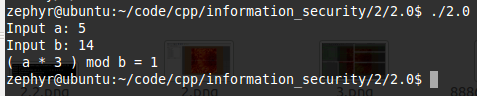
\includegraphics[width=\textwidth]{2.0.png}
\caption{扩展的Euclid算法求乘法逆元的运行结果}
\label{fig: rlt1}
\end{figure}
\end{center}

\section{编程实现换位密码}

\subsection{列换位密码}
\subsubsection{代码清单}
\begin{center}
\begin{lstlisting}[caption = {列换位密码的C++实现}, label = {lst: code2}]
template<typename T>
void display(const vector<T>& v){
  for_each(v.begin(), v.end(),
    [](T t){
      cout << t << " ";
    });
  cout << endl;
}

int main(int argc, char** argv){
  string plaintext, ciphertext;
  int column;
  cout << "Input plaintext: ";
  cin >> plaintext;
  // plaintext = "datasecurity";
  cout << "Input column number: ";
  cin >> column;
  vector<int> permutation(column);
  cout << "Input a permutation of { 1, ... , " << column << " }: ";
  for(size_t i = 0; i < column; ++i){
    cin >> permutation[i];
  }
  int dist = 26;
  int row = plaintext.size() / column;
  if(row * column != plaintext.size()){
    ++row;
  }
  int n = row * column;
  for(size_t i = 0; i < column; ++i){
    int m = 26, idx;
    for(size_t j = 0; j < permutation.size(); ++j){
      if(permutation[j] >= 0 && permutation[j] < m){
        idx = j;
        m = permutation[j];
      }
    }
    permutation[idx] = -1;
    for(auto p = plaintext.begin() + idx;;){
      int d = p - plaintext.begin();
      if(d < plaintext.size()){
        ciphertext.push_back(*p);
      }else if(d < n){
        ciphertext.push_back('z');
      }
      if(d < n){
        p += column;
      }else{
        break;
      }
    }
  }
  cout << "Ciphertext is: " << ciphertext << endl;
  return 0;
}
\end{lstlisting}
\end{center}

\subsubsection{说明}
从键盘读入矩阵的列数column、明文和一个$(1, 2, \cdots , column)$的置换$(\pi_1, \pi_2, \cdots, \pi_{column})$,输出密文,若明文无法刚好填满矩阵,则补x

置换$(\pi_1, \pi_2, \cdots, \pi_{column})$指明将明文排成column列的矩阵后,输出密文的列顺序

\subsubsection{运行结果}
\begin{center}
\begin{figure}[htbp]
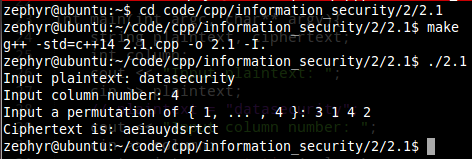
\includegraphics[width=\textwidth]{2.1.png}
\caption{列换位算法的运行结果}
\label{fig: rlt2}
\end{figure}
\end{center}

\subsection{周期换位密码}
\subsubsection{代码清单}
\begin{center}
\begin{lstlisting}[caption = {周期换位密码的C++实现}, label = {lst: code3}]
int main(int argc, char** argv){
  int d;
  cout << "Input period: ";
  cin >> d;
  vector<int> f(d);
  cout << "Input a permutation of { 1, ... , " << d << " }: ";
  for(int i = 0; i < d; ++i){
    cin >> f[i];
  }
  string m, c;
  cout << "Input plaintext: ";
  cin >> m;
  c.resize(m.size());
  for(size_t i = 0; i < m.size(); ++i){
    c.push_back(m[f[i % d] + floor(i / d) * d - 1]);
  }
  cout << "Ciphertext is: " << c << endl;
  return 0;
}
\end{lstlisting}
\end{center}

\subsubsection{说明}
从键盘输入明文、周期长度d和一个$(1, 2, \cdots , d)$的置换$(\pi_1, \pi_2, \cdots, \pi_{d})$,将密文打印在屏幕上。函数$f(i)=\pi_i$表示明文的第$i$个字母是密文中第$f(i)$个字母。则我们容易得到如下公式
\[ C[i] = M\left[ f\left( i \mod 4 \right) + \left \lfloor \dfrac{i}{d} \right \rfloor \cdot d \right] \]

其中$C$为密文,$M$为明文

\subsubsection{运行结果}
见图\ref{fig: rlt3}
\begin{center}
\begin{figure}[htbp]
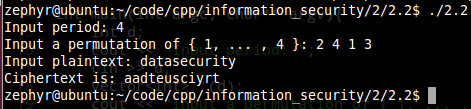
\includegraphics[width=\textwidth]{2.2.png}
\caption{周期换位算法的运行结果}
\label{fig: rlt3}
\end{figure}
\end{center}

\section{举例说明Legendre符号的作用}
\begin{enumerate}
\item 验证$a$是否是模$p$的二次剩余。若$L(a, p)=1$,则$a$是模$p$的二次剩余,否则不是
\item Jacobi符号是Legendre符号的扩展,它是通过Legendre符号来计算的。\\
\begin{enumerate}
\item $n$为素数,则$J(a, n)=L(a, n)$
\item $n$为合数,则$J(a, n)=\prod_{i = 1}^m L(a, p_i)$,其中$n$因数分解为$\prod_{i = 1}^m p_i$
\end{enumerate}
\item 在Solovay-Strassen素性测试和Rabin-Miller素性测试中均用到了Legendre符号或Jacobi符号
\end{enumerate}

\end{document}
